\section{Marco Conceptual}

\subsection{Ómicas y multiómicas}
Las ciencias ómicas engloban el estudio a gran escala de diferentes tipos de moléculas biológicas, proporcionando una visión completa de un organismo al analizar sus sistemas genéticos, moleculares y metabólicos, permitiendo descubrir cómo estos componentes interactúan y contribuyen a la salud, la enfermedad y las respuestas ambientales \cite{SilicoGene_2024} \cite{Yamada_Okada_Wang_Basak_Koyama_2021} \cite{ExplainAIMethsMultiOmics}. Entre las disciplinas principales se encuentran:

\begin{itemize}
    \item \textbf{Genómica}: analiza la secuencia, estructura y variación del genoma completo, permitiendo identificar variantes asociadas a fenotipos y enfermedades.
    \item \textbf{Transcriptómica}: cuantifica el conjunto completo de moléculas de ARN transcritas (transcriptoma) para estudiar la dinámica de la expresión génica bajo distintas condiciones.
    \item \textbf{Proteómica}: caracteriza el proteoma, es decir, todas las proteínas expresadas y sus modificaciones post‑traduccionales, clave para entender la función celular y las interacciones proteína–proteína.
    \item \textbf{Metabolómica}: mide metabolitos de bajo peso molecular, ofreciendo una instantánea del estado bioquímico y fisiológico de células y tejidos.
    \item \textbf{Epigenómica}: investiga las modificaciones químicas del ADN y de las histonas (por ejemplo, metilación y acetilación) que regulan la expresión génica sin alterar la secuencia primaria del ADN.
\end{itemize}

La \textbf{multiómica} integra dos o más de estas capas \emph{ómicas} para revelar mecanismos biológicos complejos y relaciones genotipo–fenotipo que no aparecen en estudios uniómicos aislados. Este enfoque sistémico permite, por ejemplo, identificar biomarcadores compuestos que involucran correlaciones entre variaciones genómicas, niveles de ARN, abundancia proteica y perfiles metabólicos, mejorando la comprensión de procesos tales como la progresión de enfermedades o la respuesta a tratamientos
\cite{biao2025multiomics_review}
\cite{Krassowski_Das_Sahu_Misra_2025} \cite{Vilanova2016are_multiomics_enough}.\\

\begin{figure}[h!]
  \centering
  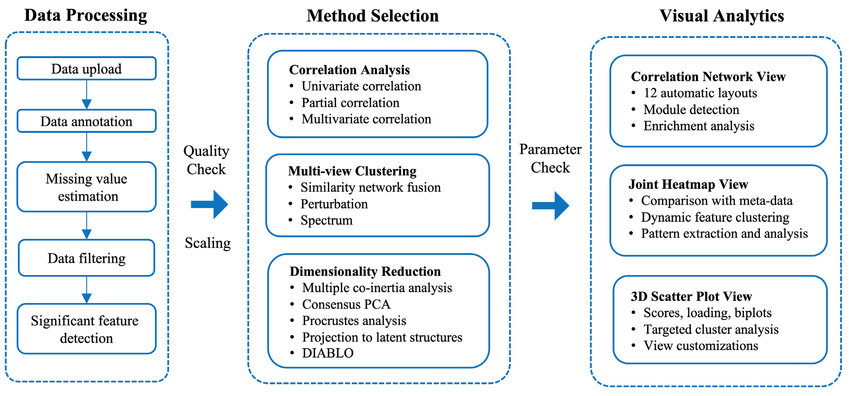
\includegraphics[scale=0.5]{images/workflow_omicsanalyst.png}
  \caption{Visión general del flujo de trabajo en OmicsAnalyst: (i) procesamiento de datos, (ii) selección de métodos de integración multivista, y (iii) análisis visual interconectado \cite{OmicsAnalyst}.}
  \label{fig:omicsanalyst_1}
\end{figure}

\newpage
La Figura~\ref{fig:omicsanalyst_1} ilustra un flujo típico de análisis multiómico incluyendo procesamiento de datos, selección de métodos (e.g., análisis de correlación, fusión de redes de similaridad, reducción de dimensionalidad como PCA/DIABLO) y visualización interactiva. OmicsAnalyst es una herramienta web ampliamente utilizada para este propósito, ofreciendo un entorno visual atractivo que facilita la integración y exploración de datos ómicos \cite{OmicsAnalyst}.\\


% ============ HACER TABLA =======================



% FLUJOS DE TRABAJO
\subsection{Flujos de trabajo multiómicos}
El análisis multiómico es un enfoque integral que combina datos provenientes de múltiples capas biológicas (genómica, transcriptómica, proteómica, metabolómica) para generar una visión holística de los sistemas biológicos. Este proceso sigue generalmente una arquitectura secuencial compuesta por etapas bien definidas, que aseguran la calidad, reproducibilidad y valor analítico de los resultados \cite{hasin2017multiomics_review} \cite{berger2021multiomics_pipeline}.

\begin{enumerate}
    % 1. Recolección y preprocesamiento de datos
    \item \textbf{Recolección y preprocesamiento de datos}
    Se inicia con la adquisición de datos ómicos desde múltiples fuentes (experimentos internos, consorcios, bases públicas), seguida de procesos de normalización, filtrado, control de calidad, estimación de valores faltantes y anotación contextual \cite{Krassowski_Das_Sahu_Misra_2025}. Cada tipo de ómica impone desafíos únicos (e.g., bajo conteo en transcriptómica, ruido técnico en metabolómica), por lo cual esta fase es crítica.

    % 2. Reducción de dimensionalidad
    \item \textbf{Reducción de dimensionalidad}
    Debido a la alta dimensionalidad típica de los datos ómicos, se aplican técnicas de reducción como \textit{Principal Component Analysis (PCA)}, \textit{t-distributed Stochastic Neighbor Embedding (t‑SNE)}, autoencoders o análisis de co-inercia múltiple. Esto permite visualizar los datos, detectar agrupamientos y mitigar la redundancia sin perder señal biológicamente relevante \cite{ramazzotti2022multiomics_dimensionality}.

    % 3. Integración de datos
    \item \textbf{Integración de datos}
    La integración puede estructurarse en tres estrategias principales:
    \begin{itemize}
        \item \textbf{Early integration:} combinación directa de las matrices, generando una única tabla combinada.
        \item \textbf{Intermediate integration:} algoritmos como \textit{MOFA}, \textit{SNF}, \textit{DIABLO} integran los datos manteniendo la identidad de cada capa y modelando relaciones latentes \cite{Argelaguet2018MOFA}.
        \item \textbf{Late integration:} cada capa se analiza por separado y los resultados se combinan en pasos posteriores.
    \end{itemize}

    % 4. Interpretación y visualización
    \item \textbf{Interpretación y visualización}
    Se exploran correlaciones, redes de interacción, firmas biológicas y relaciones funcionales utilizando herramientas como heatmaps, gráficos 3D, redes, árboles de decisión, y clústeres jerárquicos. Plataformas como \textit{OmicsAnalyst} permiten realizar estas visualizaciones de forma interactiva \cite{xia2022omicsanalyst}.

A continuación, se presenta un diagrama del pipeline en la plataforma \textit{OmicsAnalyst}, que agrupa el proceso en tres bloques principales: procesamiento de datos, selección de métodos e análisis visual interactivo (ver Figura~\ref{fig:omicsanalyst_2}):

\vspace{1em}
\begin{figure}[H]
    \centering
    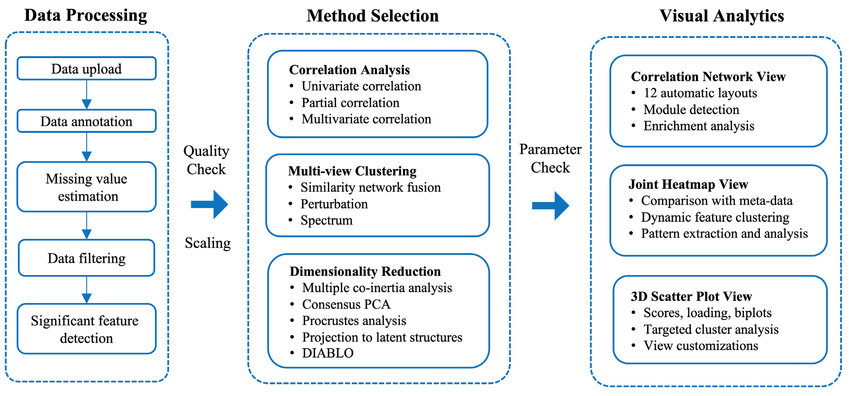
\includegraphics[width=0.9\textwidth]{images/workflow_omicsanalyst.png}
    \caption{Flujo general del análisis multiómico en OmicsAnalyst, dividido en procesamiento, selección de método y análisis visual.}
    \label{fig:omicsanalyst_2}
\end{figure}

    % 5. Ejemplos de frameworks multiómicos
    \item \textbf{Ejemplos de frameworks multiómicos}
    El uso de frameworks específicos permite automatizar y reproducir estos flujos. Por ejemplo:
    
    \begin{itemize}
      \item \textbf{MiBiOmics}: integración basada en co-inercia y redes (PCA, WGCNA) \cite{gautier2021mibiomics}.
      \item \textbf{Omix}: contiene contenedores modulares para cada etapa y modelos como \textit{MOFA+} y \textit{DIABLO}.
      \item \textbf{Holomics}: integración supervisada multietapa con enfoque modular.
    \end{itemize}
    
    \vspace{1em}
    \begin{figure}[H]
        \centering
        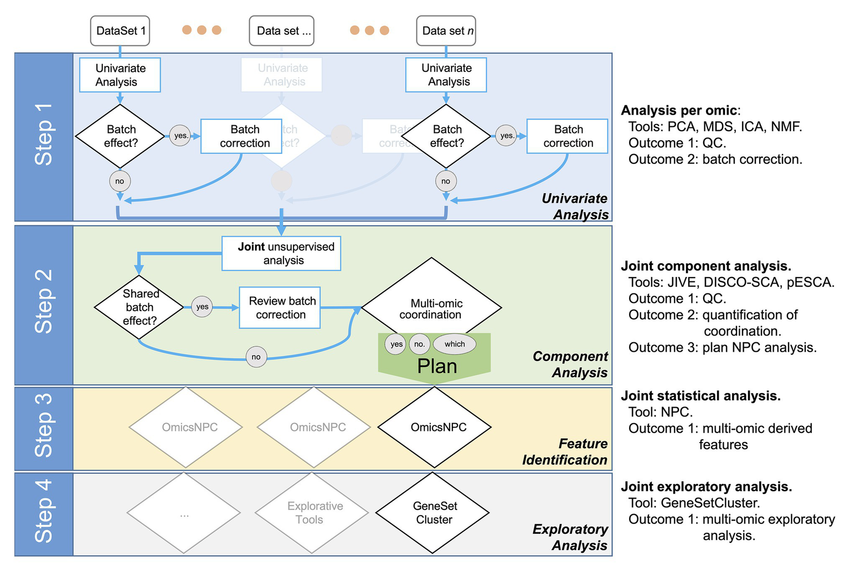
\includegraphics[width=0.95\textwidth]{images/Workflow-diagram-of-the-multi-omics-analysis-framework.png}
        \caption{Ejemplo de flujo de trabajo multiómico para análisis integrativo con pasos desde la carga hasta la fusión de datos.}
        \label{fig:workflow_framework}
    \end{figure}

    % 6. Entornos reproducibles y orquestación
    \item \textbf{Entornos reproducibles y orquestación}
    La implementación de herramientas como Nextflow y Airflow permite definir flujos de trabajo declarativos, modulares y reproducibles, integrando contenedores como Docker o Singularity junto con control de versiones. Esta capacidad resulta crítica en escenarios multiómicos, donde se manipulan datos heterogéneos, de alta dimensionalidad y alta variabilidad técnica \cite{di_tommaso2017nextflow} \cite{ewels2020nfcore} \cite{yasmin2024empirical}.\\

    Más allá de su función operativa, estos sistemas de orquestación representan una arquitectura conceptual robusta capaz de transformar datos complejos en estructuras analíticas coherentes, trazables y reutilizables. Como lo demuestra el estudio empírico \cite{yasmin2024empirical}, los principales desafíos en Airflow—la definición y ejecución de DAGs y la configuración del entorno distribuido—resaltan la necesidad de este enfoque integrado. Así, se establece una base sólida para análisis avanzados con modelos de aprendizaje automático, descubrimiento de biomarcadores, visualización integrada y toma de decisiones científicamente informada.


\end{enumerate}











% \begin{enumerate}
%   \item \textbf{Recolección y preprocesamiento de datos}: incluye la obtención de datos desde diversas ómicas (genómica, transcriptómica, proteómica, metabolómica), seguidos de limpieza, normalización, filtrado de valores faltantes y control de calidad de cada capa de datos \cite{Lehmann2020multiomics_metabolomics_review} \cite{Krassowski2020multiomics_review}.

%   \item \textbf{Reducción de dimensionalidad}: es la aplicación de técnicas como \emph{PCA}, \emph{t‑SNE}, autoencoders o análisis de componentes latentes para reducir el número de variables sin perder información relevante \cite{Tomazou2021multiomics_covid}.

%   \item \textbf{Integración de datos:}  
%     Estrategias según el momento de fusión:
%     \begin{itemize}
%       \item \emph{Early integration}: concatenación directa de las matrices ómicas.
%       \item \emph{Intermediate integration}: métodos conjuntos como MOFA o Similarity Network Fusion (SNF) para capturar factores latentes sin concatenar directamente las matrices \cite{Lehmann2020multiomics_metabolomics_review}.
%       \item \emph{Late integration}: análisis independientes por capa, combinando resultados en etapas finales.
%     \end{itemize}

%     \item \textbf{Interpretación biológica y visualización}: Identificación de biomarcadores y patrones biológicos a través de análisis estadísticos, redes de correlación y visualizaciones interactivas (heatmaps, gráficos 3D), facilitadas por plataformas como OmicsAnalyst \cite{OmicsAnalyst}\cite{Planell2021stategra}.
% \end{enumerate}

% Un resumen visual de este pipeline se muestra en la Figura~\ref{fig:omicsanalyst_2}, tomada de OmicsAnalyst, que divide el proceso en tres fases clave: procesamiento de datos, selección de métodos y análisis visual interactivo:

% \begin{figure}[h!]
%     \centering
%     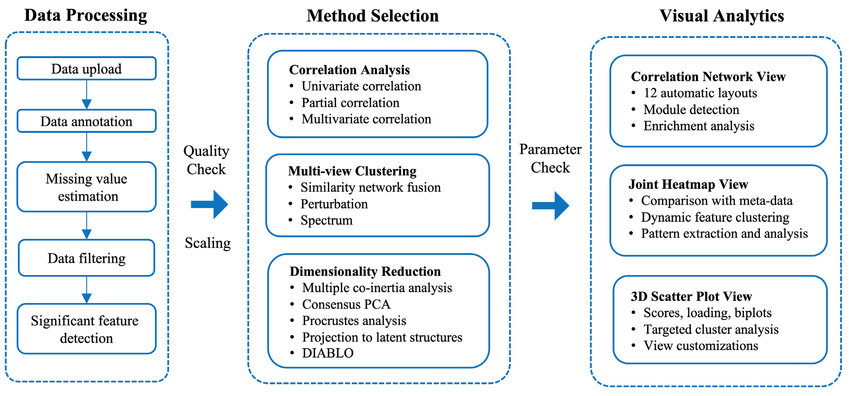
\includegraphics[width=0.8\textwidth]{images/workflow_omicsanalyst}
%     \caption{Flujo general del pipeline multiómico en la plataforma OmicsAnalyst: procesamiento, integración y visualización interactiva.}
%     \label{fig:omicsanalyst_2}
% \end{figure}

% \medskip

% \textbf{Ejemplos de herramientas y frameworks}:  
% Plataformas como \textit{Holomics} integran workflows tipo Holomics: carga de datos, análisis uniómico inicial y análisis multiómico supervisado (DIABLO o similares) en tres etapas principales \cite{turn0search3}. Aplicaciones como MiBiOmics permiten ejecutar preprocesamiento, análisis exploratorio (PCA, WGCNA), y finalmente integración multiómica basada en co-inercia o redes \cite{turn0search0}. Herramientas como Omix estructuran el pipeline en contenedores multimodales, procesamiento, análisis por ómica y fusión vertical con modelos como MOFA o DIABLO, seguidos de análisis funcionales downstream \cite{turn0search2}.


% \medskip

% \textbf{Importancia de orquestadores y entornos reproducibles}:  
% Sistemas como \textit{Nextflow} o \textit{nf‑core} permiten construir pipelines reproducibles y escalables, portables a diferentes infraestructuras computacionales, cuidando versiones, contenedores y trazabilidad técnica \cite{turn0search14} \cite{turn0search6}. Esto es especialmente útil en análisis complejos con múltiples muestras y tecnologías ómicas.

% \medskip

% Este pipeline no es solo una secuencia técnica, sino una arquitectura conceptual que permite transformar datos heterogéneos y de alta dimensionalidad en conocimiento integrable y visualizable. Así, se establece una base sólida para respaldar análisis posteriores de IA, descubrimiento de biomarcadores y toma de decisiones fundamentadas en datos.


% % Origen y aplicaciones de datos multiómicos
% \subsection{Origen y aplicaciones de datos multiómicos}
% Las fuentes de datos incluyen muestras clínicas, modelos celulares/animales, y repositorios públicos como MetaboLights \cite{yurekten2024metabolights}.

% \subsection{Principios FAIR y calidad de datos}
% Los datos multiómicos deben cumplir con los principios FAIR estableciendo identificadores únicos, APIs estándar, vocabularios controlados y metadatos ricos \cite{wilkinson2016fair_principles}. Esto exige:

% \begin{itemize}
%   \item Identificadores únicos (p.ej. DOI, UUID).
%   \item APIs REST o FTP para interoperabilidad.
%   \item Ontologías estandarizadas y metadatos enriquecidos.
%   \item Licencias y datos lisibles por máquina \cite{wilkinson2016fair_principles}.
% \end{itemize}

% \subsection{IA explicable (XAI) en entornos multiómicos}
% Técnicas como SHAP y LIME permiten entender las predicciones de modelos complejos, otorgando transparencia y respaldo científico en aplicaciones biomédicas \cite{salih2023perspective_shap_lime}.

% \subsection{Gestión documental integrada}
% Para documentar flujos de datos multiómicos es esencial un repositorio compatible FAIR, combinado con ELN/LIMS, contenedores y orquestación de pipelines mediante Airflow o Nextflow.

